\section{문제 인식과 동기}

\subsection{교육 현장의 실제 문제}

교육 현장에서 선생님들이 직면하는 가장 큰 문제 중 하나는 채점 업무의 과중함입니다. 특히 수학 과목의 경우, 답뿐만 아니라 학생들의 풀이 과정을 세밀하게 검토해야 하기 때문에 상당한 시간이 소요됩니다. 
  실제로 Quora 사이트에 올라온 How much time does it take for a teacher to grade papers?(교사가 시험지를 채점하는데 걸리는 시간은 얼마나 되나요?)라는 질문에 대해 많은 교사들이 답변을 남겼습니다. 경우에 따라 다르긴 하지만, 대체로 오랜 시간이 걸린다는 의견이 지배적이었습니다.
\begin{figure}[H]
    \centering
    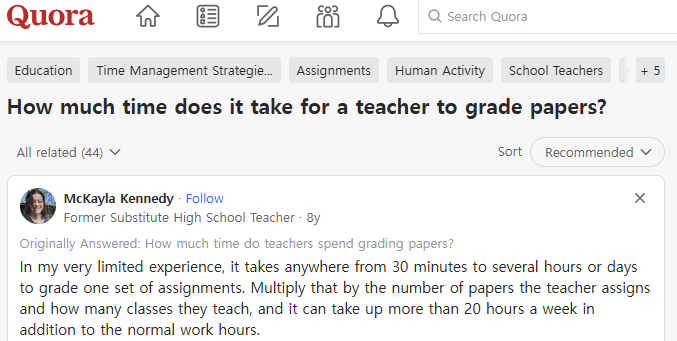
\includegraphics[width=0.5\textwidth]{1/image03.png}
    \caption{교사들의 채점 업무 현황}
    \label{fig:teacher_workload}
\end{figure}

한 명의 수학 교사가 담당하는 학생 수가 적지 않기에, 매주 숙제와 시험을 채점하는 데만 상당한 시간을 할애합니다. 이는 교사들이 수업 준비와 학생 상담에 할애할 수 있는 시간을 크게 줄이는 요인이 됩니다.

\subsection{민원 처리 문제}

\begin{figure}[H]
    \centering
    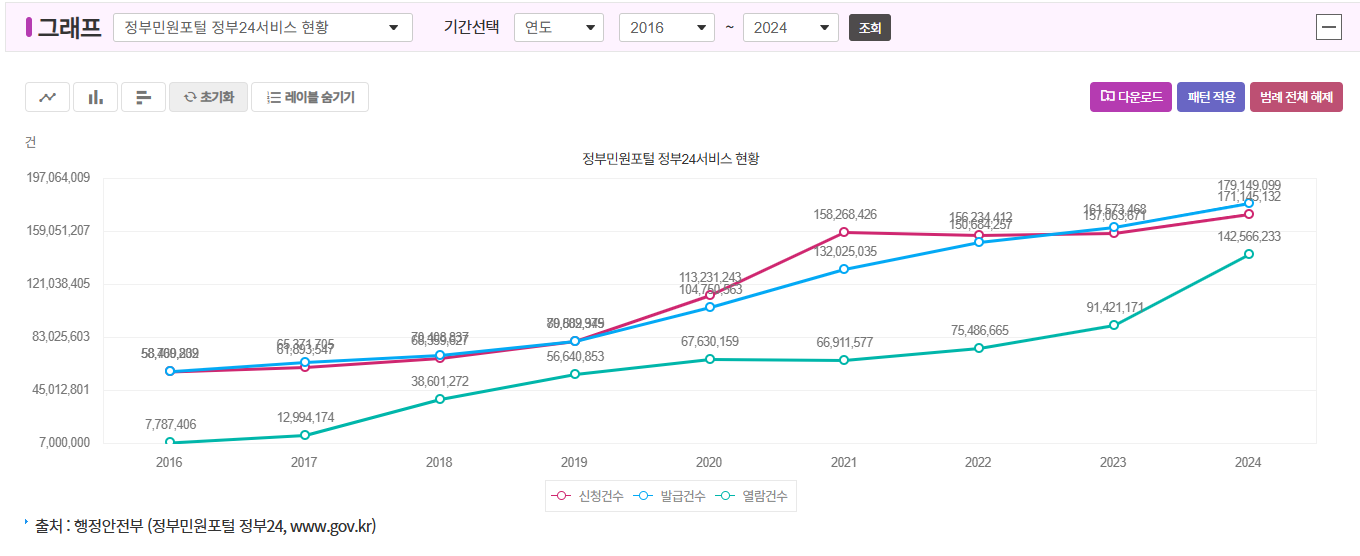
\includegraphics[width=0.5\textwidth]{1/image06.png}
    \caption{연도별 정부24서비스 민원 신청/발급/열람 건수}
    \label{fig:kiosk_elderly_struggle}
\end{figure}
 정부24서비스가 확대됨에 따라 국민들의 민원신청건 또한 증가하고 있습니다. 하루 평균 수만 건 이상의 민원이 접수 됨에 따라 공무원들의 업무 과중과 처리 지연 문제도 함께 떠오르며 국민들의 불만이 쌓여 가고 있습니다. 상당한 양의 민원을 처리해야 하는 현실, 복잡한 법령 때문에 답변을 기다리는 시민들의 불편함을 AI 기술로 해결할 수 있다고 생각했습니다.

특히 2025년 초고령사회 진입과 지방소멸 위기 속에서, 한정된 행정 인력으로 증가하는 민원 수요(연평균 15\% 증가)를 감당하는 것은 더 이상 불가능한 상황입니다. 기존에 있는 단순화된 챗봇은 정형화된 FAQ만 처리할 뿐, ``복지 수혜 자격이 어떻게 되나요?'' 같은 복잡한 질의는 전혀 이해하지 못했습니다.

\subsection{디지털 격차와 소외 계층}

또 다른 문제는 디지털 격차로 인한 소외 계층의 발생입니다. 키오스크가 보편화되면서 디지털 기기에 익숙하지 않은 사람들, 특히 노년층이 일상생활에서 불편을 겪는 경우가 늘어났습니다.

\begin{figure}[H]
    \centering
    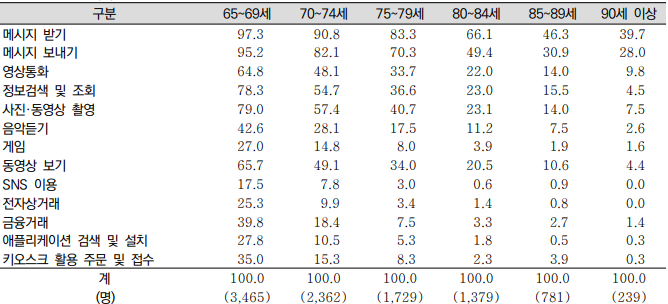
\includegraphics[width=0.5\textwidth]{1/image4.png}
    \caption{연령대별 키오스크 사용 어려움 비율}
    \label{fig:digital_divide}
\end{figure}
 지난해 한국보건사회연구원에서 발표한 '2023 노인실태조사' 보고서에서 65세 이상 노인들의 키오스크 활용 능력이 현저히 낮음을 확인할 수 있습니다.
 따라서 신속하게 민원을 처리함과 동시에 노년층의 키오스크 접근성을 확대 시킬 수 있는 방안을 고민할 필요가 있다고 생각했습니다.
 
\subsection{AI 기술의 가능성}

이러한 문제들을 해결하기 위해 AI와 LLM API를 활용한 솔루션을 개발하기로 결정했습니다. 최신 AI 기술은 이미지 인식, 자연어 처리, 대화형 인터페이스 등에서 인간 수준의 성능을 보이고 있어, 교육과 접근성 문제를 해결할 수 있는 충분한 잠재력을 가지고 있습니다.